% Options for packages loaded elsewhere
% Options for packages loaded elsewhere
\PassOptionsToPackage{unicode}{hyperref}
\PassOptionsToPackage{hyphens}{url}
\PassOptionsToPackage{dvipsnames,svgnames,x11names}{xcolor}
%
\documentclass[
  11pt,
]{article}
\usepackage{xcolor}
\usepackage[top=1in,bottom=1in,left=0.75in,right=0.75in]{geometry}
\usepackage{amsmath,amssymb}
\setcounter{secnumdepth}{5}
\usepackage{iftex}
\ifPDFTeX
  \usepackage[T1]{fontenc}
  \usepackage[utf8]{inputenc}
  \usepackage{textcomp} % provide euro and other symbols
\else % if luatex or xetex
  \usepackage{unicode-math} % this also loads fontspec
  \defaultfontfeatures{Scale=MatchLowercase}
  \defaultfontfeatures[\rmfamily]{Ligatures=TeX,Scale=1}
\fi
\usepackage{lmodern}
\ifPDFTeX\else
  % xetex/luatex font selection
\fi
% Use upquote if available, for straight quotes in verbatim environments
\IfFileExists{upquote.sty}{\usepackage{upquote}}{}
\IfFileExists{microtype.sty}{% use microtype if available
  \usepackage[]{microtype}
  \UseMicrotypeSet[protrusion]{basicmath} % disable protrusion for tt fonts
}{}
\makeatletter
\@ifundefined{KOMAClassName}{% if non-KOMA class
  \IfFileExists{parskip.sty}{%
    \usepackage{parskip}
  }{% else
    \setlength{\parindent}{0pt}
    \setlength{\parskip}{6pt plus 2pt minus 1pt}}
}{% if KOMA class
  \KOMAoptions{parskip=half}}
\makeatother
% Make \paragraph and \subparagraph free-standing
\makeatletter
\ifx\paragraph\undefined\else
  \let\oldparagraph\paragraph
  \renewcommand{\paragraph}{
    \@ifstar
      \xxxParagraphStar
      \xxxParagraphNoStar
  }
  \newcommand{\xxxParagraphStar}[1]{\oldparagraph*{#1}\mbox{}}
  \newcommand{\xxxParagraphNoStar}[1]{\oldparagraph{#1}\mbox{}}
\fi
\ifx\subparagraph\undefined\else
  \let\oldsubparagraph\subparagraph
  \renewcommand{\subparagraph}{
    \@ifstar
      \xxxSubParagraphStar
      \xxxSubParagraphNoStar
  }
  \newcommand{\xxxSubParagraphStar}[1]{\oldsubparagraph*{#1}\mbox{}}
  \newcommand{\xxxSubParagraphNoStar}[1]{\oldsubparagraph{#1}\mbox{}}
\fi
\makeatother


\usepackage{longtable,booktabs,array}
\usepackage{calc} % for calculating minipage widths
% Correct order of tables after \paragraph or \subparagraph
\usepackage{etoolbox}
\makeatletter
\patchcmd\longtable{\par}{\if@noskipsec\mbox{}\fi\par}{}{}
\makeatother
% Allow footnotes in longtable head/foot
\IfFileExists{footnotehyper.sty}{\usepackage{footnotehyper}}{\usepackage{footnote}}
\makesavenoteenv{longtable}
\usepackage{graphicx}
\makeatletter
\newsavebox\pandoc@box
\newcommand*\pandocbounded[1]{% scales image to fit in text height/width
  \sbox\pandoc@box{#1}%
  \Gscale@div\@tempa{\textheight}{\dimexpr\ht\pandoc@box+\dp\pandoc@box\relax}%
  \Gscale@div\@tempb{\linewidth}{\wd\pandoc@box}%
  \ifdim\@tempb\p@<\@tempa\p@\let\@tempa\@tempb\fi% select the smaller of both
  \ifdim\@tempa\p@<\p@\scalebox{\@tempa}{\usebox\pandoc@box}%
  \else\usebox{\pandoc@box}%
  \fi%
}
% Set default figure placement to htbp
\def\fps@figure{htbp}
\makeatother





\setlength{\emergencystretch}{3em} % prevent overfull lines

\providecommand{\tightlist}{%
  \setlength{\itemsep}{0pt}\setlength{\parskip}{0pt}}



 


\makeatletter
\@ifpackageloaded{caption}{}{\usepackage{caption}}
\AtBeginDocument{%
\ifdefined\contentsname
  \renewcommand*\contentsname{Table of contents}
\else
  \newcommand\contentsname{Table of contents}
\fi
\ifdefined\listfigurename
  \renewcommand*\listfigurename{List of Figures}
\else
  \newcommand\listfigurename{List of Figures}
\fi
\ifdefined\listtablename
  \renewcommand*\listtablename{List of Tables}
\else
  \newcommand\listtablename{List of Tables}
\fi
\ifdefined\figurename
  \renewcommand*\figurename{Figure}
\else
  \newcommand\figurename{Figure}
\fi
\ifdefined\tablename
  \renewcommand*\tablename{Table}
\else
  \newcommand\tablename{Table}
\fi
}
\@ifpackageloaded{float}{}{\usepackage{float}}
\floatstyle{ruled}
\@ifundefined{c@chapter}{\newfloat{codelisting}{h}{lop}}{\newfloat{codelisting}{h}{lop}[chapter]}
\floatname{codelisting}{Listing}
\newcommand*\listoflistings{\listof{codelisting}{List of Listings}}
\makeatother
\makeatletter
\makeatother
\makeatletter
\@ifpackageloaded{caption}{}{\usepackage{caption}}
\@ifpackageloaded{subcaption}{}{\usepackage{subcaption}}
\makeatother
\usepackage{bookmark}
\IfFileExists{xurl.sty}{\usepackage{xurl}}{} % add URL line breaks if available
\urlstyle{same}
\hypersetup{
  pdftitle={Setting Priors in brms},
  pdfauthor={Job Schepens},
  colorlinks=true,
  linkcolor={blue},
  filecolor={Maroon},
  citecolor={Blue},
  urlcolor={Blue},
  pdfcreator={LaTeX via pandoc}}


\title{Setting Priors in brms}
\usepackage{etoolbox}
\makeatletter
\providecommand{\subtitle}[1]{% add subtitle to \maketitle
  \apptocmd{\@title}{\par {\large #1 \par}}{}{}
}
\makeatother
\subtitle{Bayesian Mixed Effects Models with brms for Linguists}
\author{Job Schepens}
\date{2026-05-05}
\begin{document}
\maketitle

\renewcommand*\contentsname{Table of contents}
{
\hypersetup{linkcolor=}
\setcounter{tocdepth}{3}
\tableofcontents
}

\section{Setting Priors in brms (20
min)}\label{setting-priors-in-brms-20-min}

\subsection{Default vs.~Weakly Informative
Priors}\label{default-vs.-weakly-informative-priors}

brms uses weakly informative priors by default (not completely flat).
However, for psycholinguistics, domain-specific priors are even better.

\subsubsection{What is a Prior?}\label{what-is-a-prior}

A prior encodes your beliefs about parameter values \textbf{before}
seeing the data. In Bayesian inference:

\[\text{posterior} \propto \text{likelihood} \times \text{prior}\]

\textbf{Types of priors:}

\begin{itemize}
\tightlist
\item
  \textbf{Flat priors}: No information - any value equally likely (bad:
  implies ignorance)
\item
  \textbf{Weakly informative}: Gentle regularization - allows data to
  dominate
\item
  \textbf{Domain-specific}: Based on domain knowledge - prevents
  unreasonable values
\end{itemize}

\subsubsection{The Intercept Adapts to Your
Data!}\label{the-intercept-adapts-to-your-data}

This is important: The default intercept prior depends on
\texttt{mean(y)}. Let's see this in action:

Now let's check what default priors brms suggests:

\begin{verbatim}

=== DEFAULT PRIORS: Typical RT data (mean log-RT ≈ 6) ===
\end{verbatim}

\begin{verbatim}
                prior     class       coef   group resp dpar nlpar lb ub tag
               (flat)         b                                             
               (flat)         b conditionB                                  
               lkj(1)       cor                                             
               lkj(1)       cor            subject                          
 student_t(3, 6, 2.5) Intercept                                             
 student_t(3, 0, 2.5)        sd                                     0       
 student_t(3, 0, 2.5)        sd               item                  0       
 student_t(3, 0, 2.5)        sd  Intercept    item                  0       
 student_t(3, 0, 2.5)        sd            subject                  0       
 student_t(3, 0, 2.5)        sd conditionB subject                  0       
 student_t(3, 0, 2.5)        sd  Intercept subject                  0       
 student_t(3, 0, 2.5)     sigma                                     0       
       source
      default
 (vectorized)
      default
 (vectorized)
      default
      default
 (vectorized)
 (vectorized)
 (vectorized)
 (vectorized)
 (vectorized)
      default
\end{verbatim}

\begin{verbatim}


=== DEFAULT PRIORS: Extreme RT data (mean log-RT ≈ 10) ===
\end{verbatim}

\begin{verbatim}
                 prior     class       coef   group resp dpar nlpar lb ub tag
                (flat)         b                                             
                (flat)         b conditionB                                  
                lkj(1)       cor                                             
                lkj(1)       cor            subject                          
 student_t(3, 10, 2.5) Intercept                                             
  student_t(3, 0, 2.5)        sd                                     0       
  student_t(3, 0, 2.5)        sd               item                  0       
  student_t(3, 0, 2.5)        sd  Intercept    item                  0       
  student_t(3, 0, 2.5)        sd            subject                  0       
  student_t(3, 0, 2.5)        sd conditionB subject                  0       
  student_t(3, 0, 2.5)        sd  Intercept subject                  0       
  student_t(3, 0, 2.5)     sigma                                     0       
       source
      default
 (vectorized)
      default
 (vectorized)
      default
      default
 (vectorized)
 (vectorized)
 (vectorized)
 (vectorized)
 (vectorized)
      default
\end{verbatim}

\begin{verbatim}

=== Intercept Comparison ===
\end{verbatim}

\begin{verbatim}
Typical data prior:   student_t(3, 6, 2.5) 
\end{verbatim}

\begin{verbatim}
Extreme data prior:   student_t(3, 10, 2.5) 
\end{verbatim}

\begin{verbatim}
→ The intercept prior CHANGES with data scale!
\end{verbatim}

\textbf{Key insight}: The intercept prior automatically scales with your
data. This is convenient but has a problem: \textbf{if you don't specify
priors, your prior assumptions implicitly depend on how you code your
variables!}

\subsection{Default brms Priors}\label{default-brms-priors}

When you don't specify priors, brms assigns defaults:

\begin{itemize}
\tightlist
\item
  \textbf{Intercept}: \texttt{student\_t(3,\ mean(y),\ 2.5)} -
  \textbf{DATA-DEPENDENT!} Centers at your data mean

  \begin{itemize}
  \tightlist
  \item
    Adapts to your data scale automatically
  \item
    For RT data with mean(log\_rt) = 6: allows roughly 150ms-1100ms
    range
  \end{itemize}
\item
  \textbf{Slopes (b)}: \texttt{(flat)} - improper uniform prior over
  (-∞, +∞)

  \begin{itemize}
  \tightlist
  \item
    No information: any effect size equally likely
  \item
    Technically improper (doesn't integrate to 1)
  \end{itemize}
\item
  \textbf{Sigma} (residual SD): \texttt{student\_t(3,\ 0,\ 2.5)} with
  lower bound 0

  \begin{itemize}
  \tightlist
  \item
    Weakly informative for residual variance
  \end{itemize}
\item
  \textbf{SD} (random effects): \texttt{student\_t(3,\ 0,\ 2.5)} with
  lower bound 0

  \begin{itemize}
  \tightlist
  \item
    Encourages moderate between-subject/item variation
  \end{itemize}
\item
  \textbf{Cor} (correlations): \texttt{lkj(1)} - uniform over all
  correlation matrices
\end{itemize}

\subsection{Setting Weakly Informative Priors for Reaction
Times}\label{setting-weakly-informative-priors-for-reaction-times}

For psycholinguistics, it's better to specify priors based on domain
knowledge:

\begin{verbatim}
Our weakly informative priors:
\end{verbatim}

\begin{verbatim}
          prior     class coef group resp dpar nlpar   lb   ub tag source
 normal(6, 1.5) Intercept                               4 <NA>       user
 normal(0, 0.5)         b                            <NA> <NA>       user
 exponential(1)     sigma                            <NA> <NA>       user
 exponential(1)        sd                            <NA> <NA>       user
         lkj(2)       cor                            <NA> <NA>       user
\end{verbatim}

\subsubsection{Why These Numbers?}\label{why-these-numbers}

\paragraph{\texorpdfstring{\texttt{normal(6,\ 1.5)} for Intercept with
\texttt{lb\ =\ 4}}{normal(6, 1.5) for Intercept with lb = 4}}\label{normal6-1.5-for-intercept-with-lb-4}

\begin{itemize}
\tightlist
\item
  \textbf{Mean = 6} on log scale → exp(6) ≈ 403ms (typical RT)
\item
  \textbf{SD = 1.5} → 95\% prior interval spans {[}3, 9{]} on log scale
\item
  \textbf{Lower bound = 4} → exp(4) ≈ 55ms (minimum physiologically
  possible motor response)

  \begin{itemize}
  \tightlist
  \item
    Without \texttt{lb}, the prior puts only \textasciitilde9\%
    probability below this threshold
  \item
    Adding \texttt{lb} makes our assumption explicit: we don't entertain
    impossibly fast RTs
  \item
    In practice, data will dominate anyway, but bounded priors clarify
    our theoretical assumptions
  \end{itemize}
\item
  But 95\% of prior \textbf{mass} is between ±1.96 × 1.5 around the mean
\item
  This puts most probability on reasonable RTs (100-1500ms), while still
  allowing outliers
\end{itemize}

\paragraph{\texorpdfstring{\texttt{normal(0,\ 0.5)} for
Effects}{normal(0, 0.5) for Effects}}\label{normal0-0.5-for-effects}

\begin{itemize}
\tightlist
\item
  \textbf{Mean = 0} (no directional assumption)
\item
  \textbf{SD = 0.5} on log scale
\item
  95\% prior interval: {[}-1, 1{]} on log scale
\item
  Translates to effect sizes of roughly ±65\% of baseline
  (multiplicative)
\item
  Or approximately ±100-150ms for typical RTs around 400-600ms
\item
  \textbf{Why not flat?} Flat priors prefer extreme effect sizes
  (counterintuitive!)
\end{itemize}

\paragraph{\texorpdfstring{\texttt{exponential(1)} for Sigma and
SD}{exponential(1) for Sigma and SD}}\label{exponential1-for-sigma-and-sd}

\begin{itemize}
\tightlist
\item
  Encourages moderate variance while allowing flexibility
\item
  Penalizes very large residual variation or random effect variance
\item
  Mean = 1 on the scale of log-RTs
\end{itemize}

\paragraph{\texorpdfstring{\texttt{lkj(2)} for
Correlations}{lkj(2) for Correlations}}\label{lkj2-for-correlations}

\begin{itemize}
\tightlist
\item
  η = 2: slight preference for correlations near 0
\item
  Skeptical of strong correlations (like perfect intercept-slope
  correlation)
\item
  If you truly expected strong correlations, you could use
  \texttt{lkj(1)} or lower
\end{itemize}

\subsubsection{Comparison: Normal
vs.~Student-t}\label{comparison-normal-vs.-student-t}

brms defaults use \texttt{student\_t(3,\ μ,\ 2.5)} which has heavier
tails than \texttt{normal()}. Why switch?

\begin{verbatim}
Tails comparison (1st and 99th percentiles):
\end{verbatim}

\begin{verbatim}
Normal(0, 0.5):        -1.55 1.56 
\end{verbatim}

\begin{verbatim}
Student-t(3) × 0.5:    -5.26 5.16 
\end{verbatim}

\begin{verbatim}
Student-t ratio:       3.3 x wider
\end{verbatim}

\begin{verbatim}
Student-t allows extreme values 2x more likely than normal!
\end{verbatim}

\pandocbounded{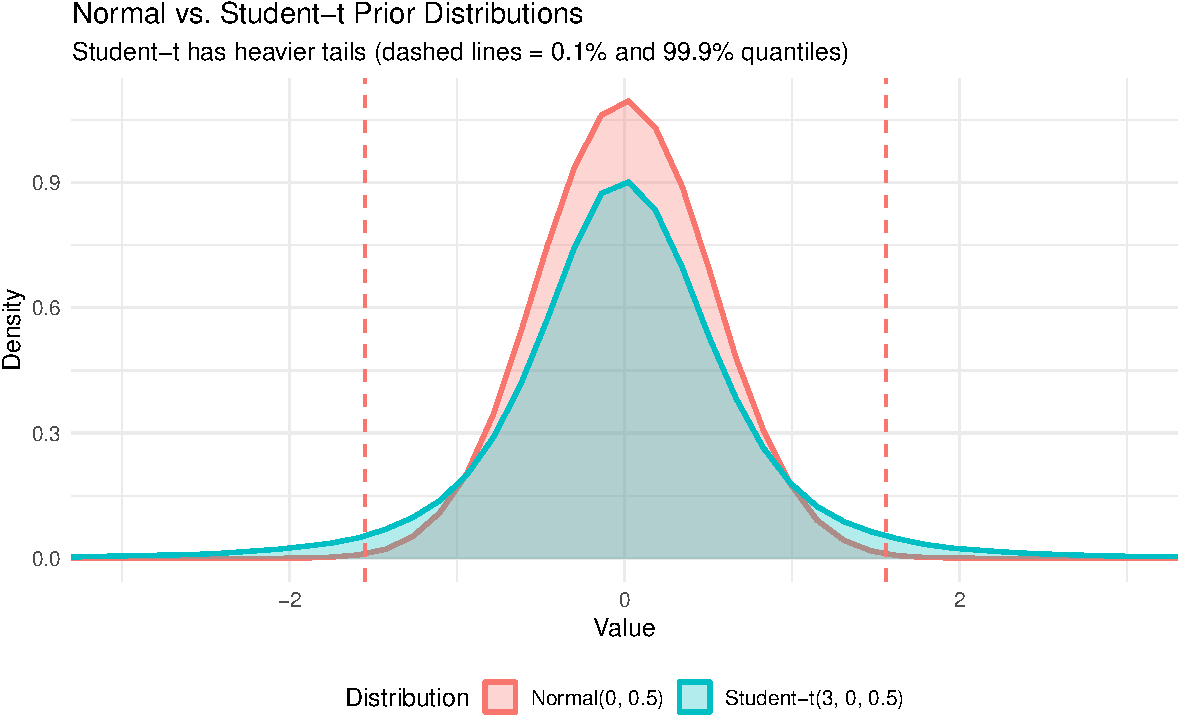
\includegraphics[keepaspectratio]{01_setting_priors_files/figure-pdf/tail-comparison-1.pdf}}

\textbf{When to use each:}

\begin{itemize}
\tightlist
\item
  \textbf{Student-t}: Default choice (conservative, robust to outliers)
\item
  \textbf{Normal}: When you have strong domain knowledge about plausible
  ranges (better for RT data in controlled experiments)
\end{itemize}

\textbf{Good sign}: Prior predictions should cover the plausible range
of your outcome variable, but not too widely.

\subsection{Summary}\label{summary}

\textbf{Key takeaways:}

\begin{enumerate}
\def\labelenumi{\arabic{enumi}.}
\tightlist
\item
  \textbf{Don't use flat priors} - they're uninformative and often lead
  to weak regularization
\item
  \textbf{Default intercept priors adapt to data} - implicit assumptions
  depend on your coding!
\item
  \textbf{Specify priors explicitly} based on domain knowledge
\item
  \textbf{Use prior predictive checks} - verify that priors generate
  plausible predictions before fitting
\item
  \textbf{Normal() is better than student\_t() when you have domain
  knowledge} - more concentrated around plausible values
\end{enumerate}

\textbf{Next steps:} - See
\texttt{02\_prior\_predictive\_checks\_rt.qmd} for detailed prior
validation - See \texttt{03\_posterior\_predictive\_checks\_rt.qmd} for
checking if the fitted model makes sense




\end{document}
